\section{Introduction}

The Republic of South Africa (RSA), often considered as the \textit{Powerhouse of Africa}, is facing many power outages or shortages of energy mainly due to the lack of investment in power infrastructure \cite{southafrica}. The RSA government is embarking on various energy and efficiency initiatives with a focus on off-grid solutions and renewable energy. The country aspires to raise an industrial revolution to shift towards a \textit{Green Economy} with the intent of boosting its manufacturing industry. This has attracted many large investors in the renewable energy sector, with the likes of Google funding Africa’s largest solar farm project in South Africa \cite{southafricarenew}.

Furthermore, the country’s ample wind resource, especially in the Western Cape and Eastern Cape regions, as seen in Figure \ref{fig:windrs} below, make it a suitable market location for the wind energy industry. Several large scale wind farms have been installed, are under construction or have been planned since 2014. The creation of the South African wind energy industry creates a market for wind turbines that are suitable for this area \cite{southafricawind}. The wind turbine designed and presented in this report will therefore be aimed at the onshore wind energy market in the Southern African region.

Most wind farms in the RSA use turbines rated between 1 and 3 MW with the most recent projects leaning towards using larger turbines of at least 2 MW. Some recent projects include \cite{southafrica}:
\begin{itemize}
    \item the Dorper WF Wind Farm, with 40 Nordex N100 Turbines rated at 2.5 MW
    \item the Dassiesklip Wind Farm, with 9 Sinovel SL3000 turbines rated at 3 MW (under construction)
    \item the Grassridge Wind Farm, with 20 Vestas V112 turbines rated at 3 MW, online since June 2015
\end{itemize}

 Considering the currently employed turbines in South Africa, the new design of turbine for this market will be adjusted so as to obtain the best economic performance; although, it is expected to fall in the power rating range of the above mentioned turbines.

%\begin{center}
\begin{figure}[H] 
%\hspace*{0}
\centering
\begin{subfigure}{0.45\textwidth}
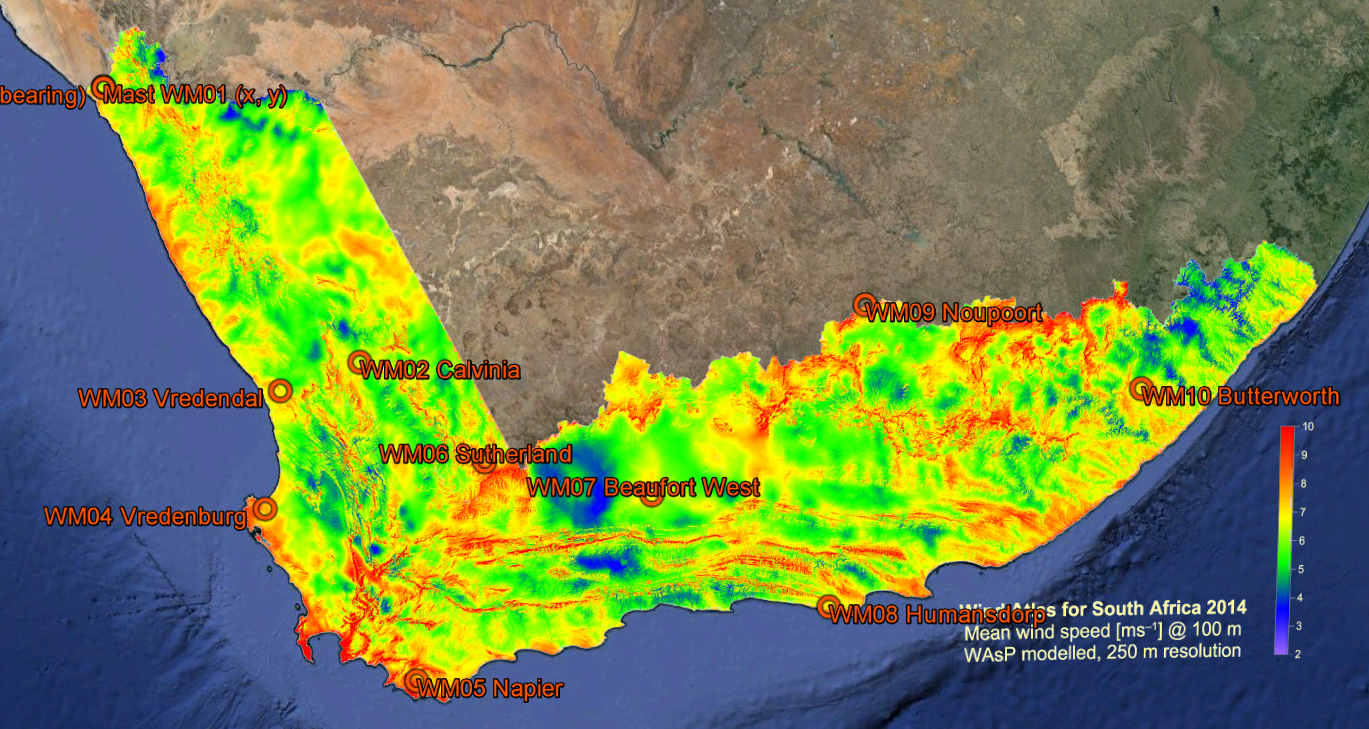
\includegraphics[width=\linewidth]{Images/Wind_atlas_map.PNG} 
\caption{South Africa}
\label{fig:windsa}
\end{subfigure}~
\begin{subfigure}{0.423\textwidth}
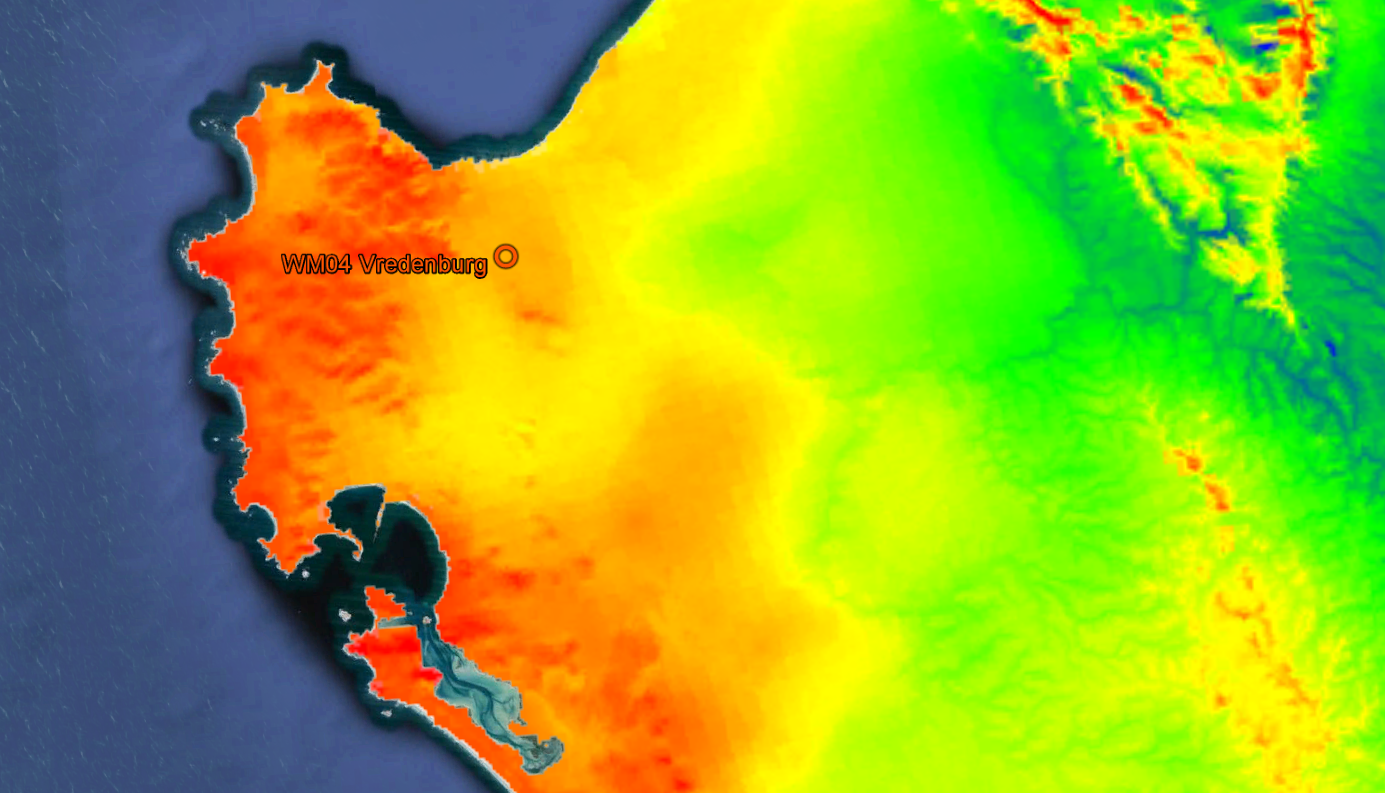
\includegraphics[width=\linewidth]{Images/Wind_atlas_zoomed.PNG}
\caption{Western Cape}
\label{fig:windlocation}
\end{subfigure}
\caption{Wind resources}
\label{fig:windrs}
\end{figure}
%\end{center}

There are currently planned projects for both onshore and offshore wind farms, thought the investment cost of a new offshore farm is still very high, on average in the range of 2.0 to 2.2 million €/MW. The construction of such a wind farm is today only possibly with the support of the government \cite{offcost}. The majority of wind turbines in South Africa today are located in the western and eastern cape regions as these areas have good wind resources. The current energy price has been found to have an average of 0.619 zar/kWh equal to 0.034 €/kWh \cite{eprice} which is an indicator for later discussion regarding the economic potential of the new wind turbine.

For assistance in the calculations of the new turbine, a 5 MW reference turbine have been used \cite{5MW}. This reference has been used to make a first assumption of size and constraints through scaling. It has also been used for guidance in the choice of design parameters and structural design.
